%!TEX root = ../thesis.tex
%*******************************************************************************
%*********************************** First Chapter *****************************
%*******************************************************************************

\chapter{Introduction}  %Title of the First Chapter

\ifpdf
     \graphicspath{{/Users/luyolomagangane/Documents/Academics/Figures/Chapter1/}}
\else
    \graphicspath{{Chapter1/Figs/Vector/}{Chapter1/Figs/}}
\fi


%********************************** %First Section  **************************************

\section{Overview} %Section - 1.1 

\emph{"... as they say, your model is only as good as the data you have. \newline So it all starts with the data ..."} \newline
\indent \indent - Nyalleng Moorosi, \emph{Deep Learning Indaba} (2017). \newline 

Artificial intelligence (AI) is the imitation of human-level intelligence by machines. Human beings are capable of extracting information from a passage of text and transforming that information into a mental model of objects and relationships between those objects. As stated by Nyalleng Moorosi, the model is only as good as the data you give it, this is true for both human mental models as well as machine constructed models. \newline 
Human models are often confined to a finite domain ~\citep{staab2010handbook}, for example a mental model might be one of the entertainment industry. The entertainment industry contains objects such as films, actors and actresses, characters and awards. These objects have relationships between them, such as "stared in", "worked along side", "a character in", and "was nominated for". Humans can use this model to easily reason about new relationships between the objects that weren't mentioned in passage of text. For example the text may say that Chadwick Boseman stared in a movie called Black Panther, and using that information we can reason that Chadwick Boseman "is an" actor. \newline
We use these models to read and understand other passages of text, in conversations with other people, and to help us answer questions. The set of objects and the relationships between them, within a domain, can be thought of as knowledge. Figure 1.1. shows what knowledge about the entertainment industry might look like. \newline

\begin{figure}
  	\caption{Objects and the Relationships between Them}
   	\centering
    	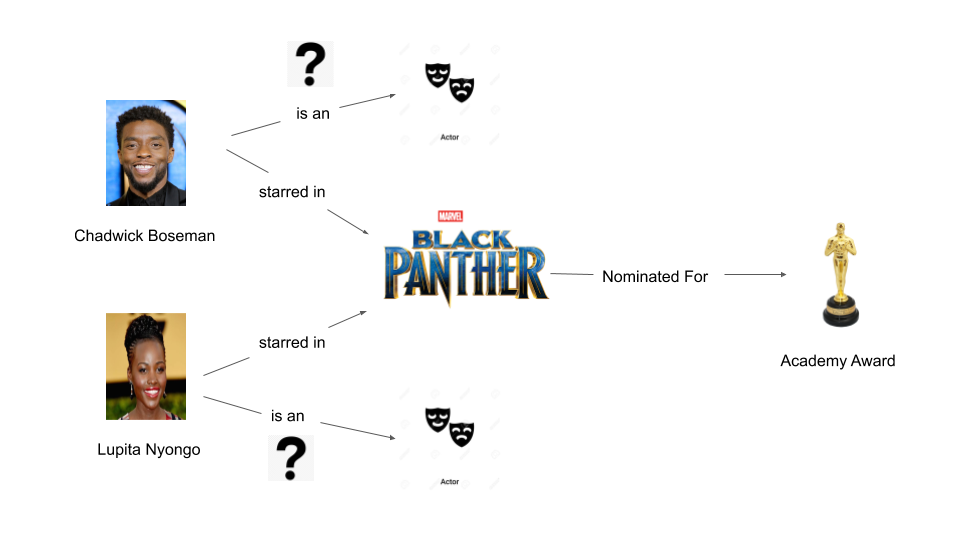
\includegraphics[width=\textwidth]{Objects_and_the_Relationships_Between_Them}
\end{figure}

\textbf{Challenges}. Reasoning about knowledge expressed in natural language ~\citep{minervini2019differentiable} is simple for humans, but trying to imitate this behaviour in computers reveals its underlying complexity. \newline 
The first task is providing a mechanism for perceiving syntax. Humans recognise text as sequences of words, and words as a sequence of characters. Characters can belong to different writing systems which can be dense - have a few characters used in a large number of combinations, or sparse - have a very large number of characters used in less combinations ~\citep{Hua2010}. A computer has to first be able to perceive these characters. \newline
The second task is even more challenging: semantics. Semantics is the meaning of words in language ~\citep{chomsky1955logical}. Semantics is what allows humans to understand each other in conversation, through written text, and through visual imagery. Semantics allow us to understand that an actor is a thing, and that things can have relationships with other things. Giving computers the capability to semantic understanding is very challenging because of the "messiness" of language. If a person is shown a word in the singular, and a word in the plural, for example "film" and "films" a person will most likely understand that there is not much difference in meaning between the two words, a computer may interpret them as having completely different meanings. Different words can also have similar meanings, for example "movie" and "film". Capturing this statistical similarity once again challenging for machines. And finally the order in which words are seen provides context, for example, the word "star" has completely different meaning in "Chadwick Boseman is a movie star" and "Black Panther looked up into the night sky an saw a star". \newline
The third task is organising information in such a way as to be able to reason about the knowledge it conveys. Humans build mental models using default reasoning ~\citep{reiter1980logic} - believing that most Objects A have relationship Relationship with Object B, with a small number of exceptions. For example we could believe that films (Object A) have not won (Relationship) an Oscar (Object B), except for films such as Black Panther (Object B). We will believe this is true for any given movie, unless we are familiar enough with movie history to identify the exceptions. Formallly, the default beliefs we hold are facts, and this process of reasoning allows us to infer new facts - plausible relationships between objects. \newline
In order to allow computers to use the same method of reasoning, data has to be structured as facts and stored in a database. Such a database is called a knowledge base (KB) ~\citep{carlson2010toward, angeli2013philosophers}  and is modelled on ontologies. A KB is used to store facts, which encode knowledge about a domain. These facts are modelled as triples - subject, predicate, object, where the subject and object are entities, and the predicate is the relation between the two entities. For example, a fact (triple) in the entertainment KB would be Black Panther (subject/entity) is a (predicate/relation) super hero (object/entity). This model is derived from the resource description framework model of the semantic web ~\citep{bizer2009dbpedia}. \newline
The problem with this approach is facts are either present in the database or they are not i.e. questions can be answered exactly, or they cannot. There is no measure of plausibility that can be used to accept new potential facts, or discard implausible facts ~\citep{koller2007introduction}. \newline
\textbf{Encourging Progress}. The task of reasoning about knowledge expressed in natural language is a daunting one, however we have seen tremendous progress in statistical relational learning. The first major progress was the integration of the bilinear tensor product and neural networks ~\citep{socher2013reasoning}. This approach effectively extended linear tensor factorisation techniques to nonlinear tensor factorisation. The approach simultaneously introduced using pre-trained word embeddings to initialise entities and relations, instead of using randomly initialised word vectors. In this one approach, both reasoning and semantic representations were extended. \newline
The second time major progress was realised was with the use of complex valued embeddings for link prediction ~\citep{trouillon2016complex}. This approach extended the Bilinear Tensor product by making use of Hermitian dot product, the complex counterpart of the standard dot product between real vectors. The approach proposes complex vectors can effectively capture antisymmetric relations while retaining the efficiency benefits of the dot product. This was achieved by using representations with complex embeddings $\mathbb{C}$, allowing the model to capture the semantic meaning depending on the order of the embeddings. \newline 
The previous two milestones relied on shallow models that could scale to large datasets. Up until that point, research in link prediction had focused on minimising the parameterisation of models. Convolutional networks are parameter efficient models, and major progress was again realised with the use of convolutional deep learning models for link prediction ~\citep{dettmers2018convolutional}. The approach makes use of 2D embedding representations which allow the modelling of a high number of interactions between embeddings. \newline 
Despite this progress, we've yet to see this method knowledge-based reasoning deployed to real-life applications. Alternative methods such as approaches to solving the Stanford Question Answering Dataset (SQuAD) ~\citep{rajpurkar2016squad}, General Language Understanding Evaluation (GLUE) benchmarks ~\citep{liu2019roberta}, and the Alexa Prize ~\citep{ram2018conversational}, have seen greater commercial adoption. Applications of link prediction seem to be more focused on the evolution of relational databases, and have so far found utility in laboratory information management systems ~\citep{HARROW20192068}. \newline
\textbf{Remaining Challenges}. Perhaps the lack of adoption in link prediction is due to the current neural factorisation model state-of-the-art (SOTA) performance in open-domain question answering: 25.20\% ~\citep{balazevic2019hypernetwork}. A possible explanation for why SOTA performance is so low is that Toutanova and Chen ~\citep{toutanova2015observed} realised inverse relation test set leakage from the training set of FB15k. Because of this test set leakage, simple rule-based models were able to exploit inverse relations in the test set and achieve SOTA performance. Similarly, current neural factorisation model SOTA performance on the less challenging WN18RR dataset is 43.60\%. Dettmers et al. ~\citep{dettmers2018convolutional} created this dataset after discovering a similar test leakage problem in WN18. We can conclude that link prediction SOTA performance has to dramatically improve before wide-spread adoption can be realised. \newline
\textbf{Outline of contributions}. SOTA neural factorisation models ~\citep{balazevic2019hypernetwork, dettmers2018convolutional} introduce relational covariate shift ~\citep{ioffe2015batch}. The models extend the bilinear model ~\citep{jenatton2012latent} by computing subject-predicate transformations using a convolutional operation ~\citep{zeiler2014visualizing}, instead of a dot product. This extension exacerbates covariate shift between the subject and predicate features. We correct for this exacerbated covariate shift by regularising relational filters using batch normalisation. \newline 
Leveraging semantic information ~\citep{NIPS2013_5028} from pre-trained word embeddings ~\citep{mikolov2013distributed} can provide richer representations which can be used for improved inference during reasoning. At the same time, link prediction benchmark datasets often only present one or two occurrences of facts, leading to limited opportunity in capturing the appropriate representation distributions for entities and relations. We integrate pre-trained word embeddings into SOTA neural factorisation model training to compensate for this sparsity in representational data, providing richer context with which to perform reasoning. \newline
\textbf{Long-term Motivations}. Reasoning about knowledge expressed in natural language is one of the strongest measures of intelligence possessed by humans. This capability allows the discourse, debate and dialogue. In order for humans to realise artificial general intelligence (AGI), this skill has to be mastered by machines. Potential applications that can be designed using such technology have profound implications for all aspects of society including in education - such as tutoring systems, health - primary health frontline assistants, and science - from applications such as astronomy to energy research. Practical implementations of AGI will be grounded in natural language and the internet. This works aims to contribute implementations that help in methodology understanding toward the realisation of full AGI.  \newline
\textbf{Short-term Motivations}. We note the poor performance in open domain question answering currently achieved by SOTA neural factorisation models ~\citep{balazevic2019hypernetwork, dettmers2018convolutional}. A sensible implementation of AGI would use heterogeneous information sources from the internet ~\citep{angeli2013philosophers}. Extracting information from the web, constructing or expanding knowledge bases, and then answering questions ~\citep{shalaby2019beyond} is currently the most successful paradigm for open domain question answering. Given the most successful models using this paradigm have poor performance, there is an opportunity to refine existing techniques in the aim to make them more useful in answering questions in this way. Revolutionising existing methods that try to solve AI tasks by making use of deep learning techniques has seen tremendous progress in fields such as computer vision ~\citep{hudson2018compositional}  and natural language processing ~\citep{peters2018deep}. Neural factorisation approaches should attempt further integration of deep learning methods, with the adoption of practices from such fields applied to training, reasoning and knowledge representation. Given that deep learning itself is modelled after human after the human mind, it seems sensible to try to bring SRL into closer alignment with methods of reasoning used by humans. \newline
\textbf{Challenges of this approach.}  In order to answer open-domain questions, the domain in which the knowledge belongs needs to be defined. Facts about that domain then need to be populated. Typically this is achieved by scanning documents written in natural language on the internet ~\citep{fader2011identifying, dong2014knowledge} and populating a knowledge base. Given the heterogeneity of these data sources, it can be difficult consolidating the information into a central datastore which can the be used to perform inference.  Related to the problem of centralising knowledge, the number of facts within a domain can range from hundreds of thousands, to millions. The poses a sample scarcity or model density problem. In the former, it becomes a challenge to adequately model the probability distributions of plausible relations given the in frequency in observations of facts about a particular subject. In the latter, the required large parameterisation of  models is needed to encode knowledge within the domain. \newline
An additional challenge to this method of question answering are the compute resources required to perform inference. For any given question, current methods perform an inference test on every entity within the knowledge base. This is not a challenge knowledge bases with a small number of entities, for example tens of thousands of entities, however this poses a serious scalability problem from knowledge bases with entities in the millions. This compute problem presents significant opportunity for more scalable inference implementations. Similarly, question answering is modelled as a classification task, where the classification categories are the entities themselves. This means small numbers of target categories are in the tens of thousands, and can be as large as millions of categories. This seems like an impractical method of modelling question answering and also presents significant opportunity for improvement. 

%********************************** %Second Section  *************************************

\section{Related Work} %Section - 1.2 
\textbf{Reasoning and natural language.} This dissertation aims to extend research that aspires to give computers the capability of human-like reasoning ~\citep{bordes2011learning} in open domain question answering ~\citep{hakimov2019evaluating}. Early work in this area focused on learning deterministic logical concepts based on symbolic frameworks ~\citep{hohenecker2017deep} which were used for formal reasoning. Later, attempts to relax formal reasoning and make use of more flexible embedding representations of natural language inspired research in statistical relational learning (SRL) ~\citep{koller2007introduction}. Link prediction is an SRL approach to human-like reasoning that makes use of knowledge bases ~\citep{balazevic2019hypernetwork, dettmers2018convolutional, socher2013reasoning}. \newline
% Modelling interactions between entities and relations
Early approaches to reasoning over facts in KBs were attempted using tensor factorisation ~\citep{nickel2011three} to model entity-relational interactions. Nicek et al. (2011) implemented RESCAL, a model that uses the bilinear tensor product to  
% Natural language representations

%********************************** % Third Section  *************************************

\section{Modelling Techniques} %Section - 1.2

\subsection{Neural Factorisation} % Latent Feature Modelling
Entities and relations are words that can be represented as real-valued vectors [references]. These real-valued vectors form part of a euclidean embedding space that represents a knowledge domain [references]. The entity and relational vectors can be randomly generated, or be pre-computed to capture semantic meaning [references]. A classification model can then be constructed that generates a probability distribution over probable facts within the knowledge domain. In order to compute the probability distribution, a number of latent feature modelling techniques are used, including tensor factorisation [references], circular correlations [reference] and convolutional feature maps [reference]. These methods can broadly be defined as linear and nonlinear. Attractive attributes of linear latent models are their simplicity, ease of implementation and computational efficiency. Linear latent models however suffer from a lack of expressiveness and struggle to model complex, contradictory or incoherent relationships between entities. Nonlinear latent feature models are able to produce more expressive latent feature sets, and so more adept at capturing complex relationships. Nonlinear models however suffer from computational inefficiency and poorly generalise concepts. \newline
\subsection{Graph Representation Learning} % Graphical Modelling
In Graph Feature Modelling, Knowledge Graphs (KG) are used to model domains. KGs are composed of nodes and edges, where nodes represent entities and edges represent relations. The graphical structure then captures local, quasi-local and global domain properties. This global structure exhibits particular properties about relations within the domain, characteristics of the entities of the domain, and local entity-relational sub-structures. These graph structure properties are used in supervised [reference] and unsupervised [Graph Infomax] settings for SRL tasks such as link prediction and entity-resolution. The directional nature of edges in graph structures (uni-relational and bi-relational) is also exploited to further enhance the fulfillment of SRL tasks [reference]. The assumption in general in KGs is that similar entities will be collocated within a local and quasi-local regions, and that global similiarty patterns between entities will be captured by the ensemble of all paths between entities. Link-based clustering [reference] is thus used at all these structural scopes, and supports link prediction and entity-resolution tasks. 
\subsection{Inductive Probabilistic Logic Programming}  % Inductive Probabilistic Logic Programming
We won't be talking about this.

%********************************** % Third Section  *************************************
\section{Link Prediction with Latent Feature Models}  %Section - 1.3 
\label{section1.3}
\subsection{Knowledge Graph Latent Feature Models}
Link prediction with latent feature models involves building entity-relational representations from the nodes and edges of knowledge graphs expressed as subject-predicate object triples. These triples explicitly model facts within a knowledge domain. Entity and relational representations are commonly implemented as real-valued vectors. The vectors are then combined using compositional models, such as neural networks, to produce latent relational representations that can be used to compute the likelihood of plausible relationships between entities. The domain can be said to represent a multidimensiona embedding space into which the entities and relations are projected. Knowledge graph based latent feature modelling approaches are similar to semantic embedding representations [rerferenc]. They differ in that knowledge graph approaches explicitly model entity-relational interactions,  and semantic embedding approaches rely on the distributional word representation techniques [reference], relying on Skip-Gram [reference] and Contious Bag of Words [reference] to generate word representations. This is an implicit modelling of relationships between word vectors. \newline
\subsection{Tensor Factorisation}
Factorisation attempts to model concepts between words, these facts are discovered using unsupervised techniques such as singular value decomposition. In the case of knowledge graphs, we obtain explicit representations of these concepts and can use them for entity-relational transformations that represent intermediate relational concepts that can then be used to determine plausible relationships when tested against subject entities.
Tensor factorisation is an approach used for link prediction with latent feature models. It involves modelling entity relationships as matrix slices that comprise a relational tensor. The entity between entities is then computed using a bilinlear tensor product [reference], where the inner product of the object entity is taken with the matrix relational representation before an inner product of the resultant representation is taken with the subject entity. Bilinear tensor factorisation models are efficient in their number of parameters but lack expressiveness. Multilayer perceptrons have been used to overcome the lack of expressiveness however often suffer from overfitting. Recently convolutional neural networks have been proposed to allow expressive factorisation [references], do not suffer from overfitting and remain computationally efficient. \newline
\subsection{Other of Latent Feature Modelling Approaches}
A number of alternative approaches to latent feature model factorisation have been proposed for link prediction, including circular correlation [reference], holographic entity-relational transformations [reference], toroidal representations [reference]. The rest of this dissertation focuses on factorisation of latent feature models, with the explicit representation of relational concepts. \newline

\nomenclature[z-DEM]{DEM}{Discrete Element Method}
\nomenclature[z-FEM]{FEM}{Finite Element Method}
\nomenclature[z-PFEM]{PFEM}{Particle Finite Element Method}
\nomenclature[z-FVM]{FVM}{Finite Volume Method}
\nomenclature[z-BEM]{BEM}{Boundary Element Method}
\nomenclature[z-MPM]{MPM}{Material Point Method}
\nomenclature[z-LBM]{LBM}{Lattice Boltzmann Method}
\nomenclature[z-MRT]{MRT}{Multi-Relaxation 
Time}
\nomenclature[z-RVE]{RVE}{Representative Elemental Volume}
\nomenclature[z-GPU]{GPU}{Graphics Processing Unit}
\nomenclature[z-SH]{SH}{Savage Hutter}
\nomenclature[z-CFD]{CFD}{Computational Fluid Dynamics}
\nomenclature[z-LES]{LES}{Large Eddy Simulation}
\nomenclature[z-FLOP]{FLOP}{Floating Point Operations}
\nomenclature[z-ALU]{ALU}{Arithmetic Logic Unit}
\nomenclature[z-FPU]{FPU}{Floating Point Unit}
\nomenclature[z-SM]{SM}{Streaming Multiprocessors}
\nomenclature[z-PCI]{PCI}{Peripheral Component Interconnect}
\nomenclature[z-CK]{CK}{Carman - Kozeny}
\nomenclature[z-CD]{CD}{Contact Dynamics}
\nomenclature[z-DNS]{DNS}{Direct Numerical Simulation}
\nomenclature[z-EFG]{EFG}{Element-Free Galerkin}
\nomenclature[z-PIC]{PIC}{Particle-in-cell}
\nomenclature[z-USF]{USF}{Update Stress First}
\nomenclature[z-USL]{USL}{Update Stress Last}
\nomenclature[s-crit]{crit}{Critical state}
\nomenclature[z-DKT]{DKT}{Draft Kiss Tumble}
\nomenclature[z-PPC]{PPC}{Particles per cell}